\section{Superhydrophobe Oberflächen}

\textbf{Was sind \glqq smart materials\grqq \dangersign?} Festkörper, Flüssigkeiten oder Gase, die selbständig auf veränderte Umwelteinflüsse reagieren (können). Ein Beispiel für ein \glqq smart material\grqq\ ist die \textbf{Cuticula}, die Grenzfläche zwischen Pflanze und Umwelt. Diese wird auch als äußere Epidermiszellwand bezeichnet. Die Cuticula findet sich in der Wachsschicht von Trauben, Lotus-Blättern und Stacheln von Kakteen. 

\subsection{Plfanzenkutikula - Funktionen und Struktur}

\begin{center}
	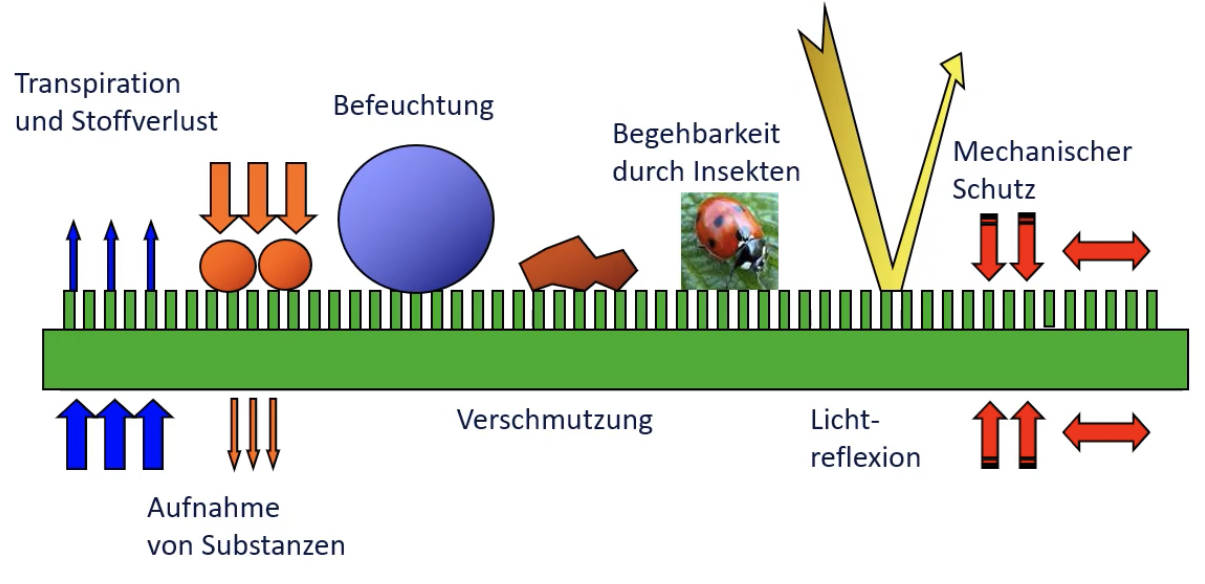
\includegraphics[width=10cm]{lec2/figures/kutikula-funktionen.png}
\end{center}
(\dangersign \textit{Nenne vier Funktionen der Pflanzenkutikula.})

\begin{itemize}
    \item Transpiration und Stoffverlust
    \item Aufnahme von Substanzen
    \item Befeuchtung
    \item (Vermeidung von) Verschmutzung
    \item Begehbarkeit durch Insekten (z.B.\ um Schädlinge zu konsumieren)
    \item Lichtreflexion (z.B.\ in Wüstenregionen bei zu starker UV-Strahlung)
    \item Mechanischer Schutz
\end{itemize}
Das Blatt besteht aus verschiedenen Zelltypen, wie in dem folgenden Querschnitt zu sehen ist. Während die Cuticula und Epidermis schützen und die Interaktion mit der Außenwelt kontrollieren, bilden die oberen Zellen eine Stützstruktur und die unteren Zellen ein Leitsystem für Wasser und Nährstoffe.
\\\\
\textit{Anmerkung: Die Komponenten des hier abgebildeten Blattquerschnitts müssen nicht auswendig gelernt werden}.

\begin{center}
	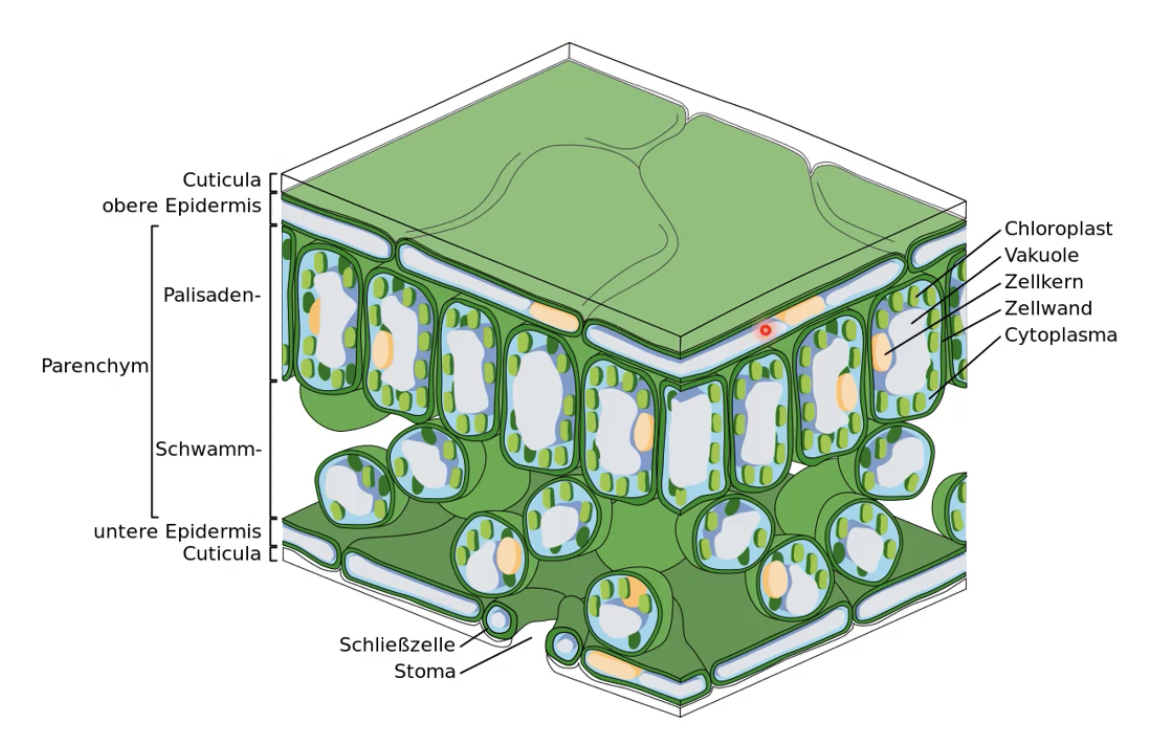
\includegraphics[width=8cm]{lec2/figures/blatt-querschnitt.png}	
\end{center}
Der \textbf{strukturelle Aufbau der Kutikula} ist idealisiert ein schichtweißer Aufbau. In der Realität handelt es sich allerdings um Verbundmaterialien, welche technisch aufwändig zu rekonstruieren sind. Die einzelnen Schichten bestehen dabei aus verschiedenen Alkoholen und Fettsäuren.

\begin{center}
	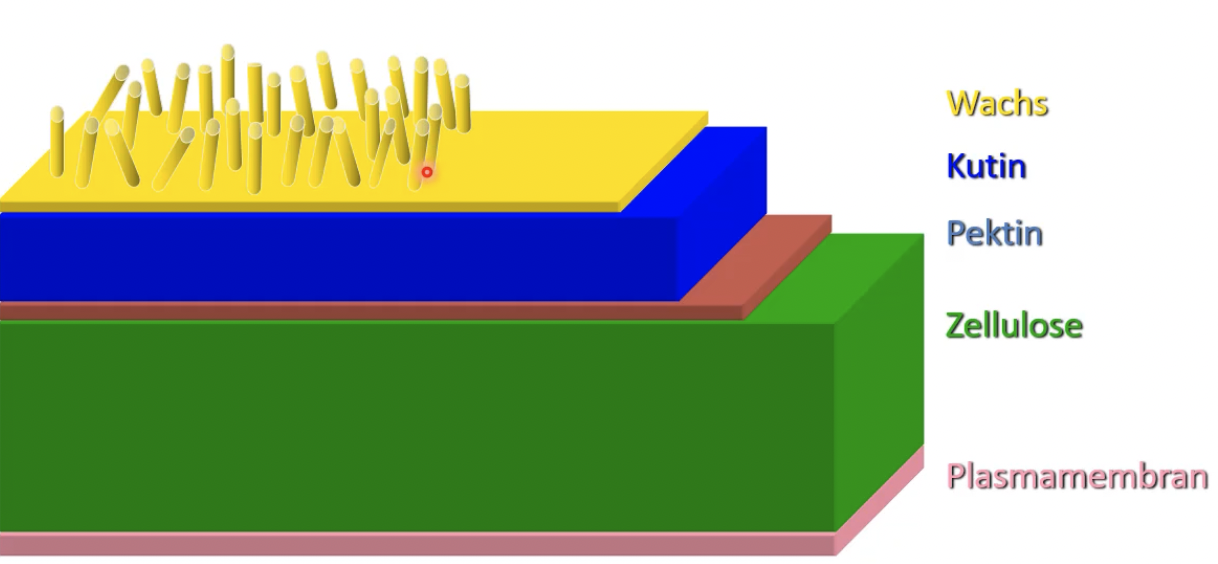
\includegraphics[width=8cm]{lec2/figures/kutikula-aufbau.png}	
\end{center}

\subsection{Messmethoden für Oberflächen}

\subsubsection{Raster-Elektronen-Mikroskop (REM)}

Das REM rastert die Obefläche der Probe mit einem sehr feinen Elektronenstrahl ab. Die Elektronen werden aus einer Elektronenquelle gewonnen, über Spulen fokussiert, beschleunigt und treffen auf die Probe auf. Die dort ausgelössten Effekte (z. B. Strahlungseffekte) werden von verschiedenen Dektoren erfasst und geben rückschlisse auf \textbf{Topografie, Materialkontrast und Zusammensetzung} der Probe. Die Rohbilder sind immer in schwarz-weiß, können aber in der Nachbearbeitung anhand der Graustufen eingefärbt werden.\\

\begin{center}
	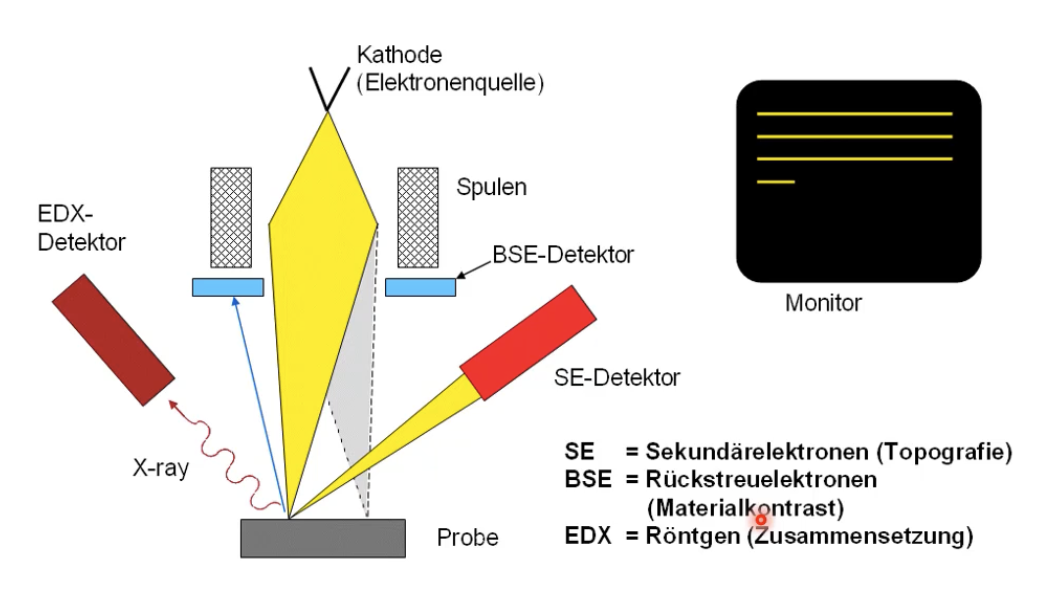
\includegraphics[width=8cm]{lec2/figures/rem.png}	
\end{center}
Um im Rahmen der bionischen Entwicklung geeignete Strukturen und Materialien zu finden, werden zunächste REM Aufnahmen verschiedener Oberflächen untersucht. Bei Pflanzen gibt es z.B.\ glatte Oberflächen, Pallisadenstrukturen und Wellenformen. Die Ausprägung der Kutikula liefert allerdings noch nicht genug Informationen darüber, ob ein gewisser Effekt durch sie bedingt ist. Daher sollten im Rahmen der bionischen Untersuchung im Stammbaum getrennte Arten mit ähnlichen Strukturen auf einen gewünschten Effekt hin getestet werden. Tritt dieser auf, so liegt die Vermutung nahe, dass die Oberfläche dafür verantwortlich ist.
\\\\
Pflanzliche Oberflächen sind oftmals rauh und haben diverse Strukturierungsmöglichkeiten mit Spalten, Fäden und Papillen (Zapfen). Auch das Wachs kann sich sehr unterschiedlich ausbilden und bietet eine Auswahl an Mikrostrukturen.

\subsubsection{Weißlicht-Profilometrie (WP)}

Bei der WP wird eine Quantifizierung der Topographie erzielt (Höhenmessung). Dafür werden Interferenzmuster ausgenutzt, um die Höhe von Mikrostrukturen auf der Oberfläche im $\mu$-meter Bereich zu messen.

\begin{center}
	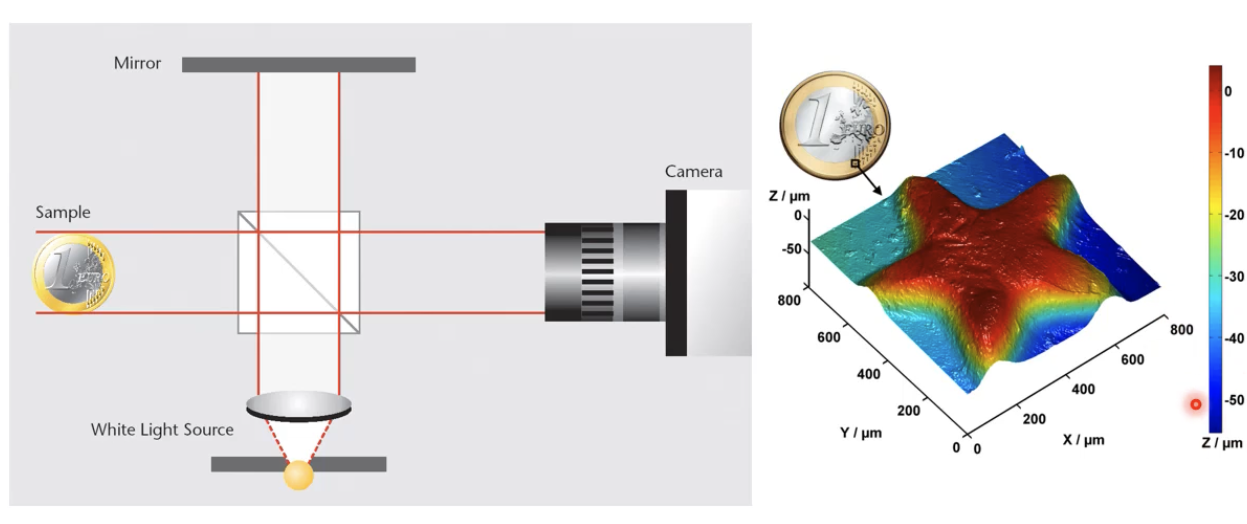
\includegraphics[width=8cm]{lec2/figures/wp.png}	
\end{center}

\subsection{Antiadhesion}

Bei wasserabweisenden Plfanzen tritt der Effekt der \textbf{Antiadhesion} auf. Die Blätter sind unbenetzbar und das Wasser perlt in Tropfen ab. Bekanntester Vertreter ist die Lotus-Pflanze. Der Effekt wurde im Rahmen der Reinigung entdeckt, welche notwendig ist, um REM-Aufnahmen der Oberfläche zu erstellen. Verantwortlich dafür ist eine hohe Rauheit und eine Papillenartige Mikrostruktur.

\subsubsection{Maße zur Beschreibung der Antiadhesion/ Benetzung}

\textbf{Rand-/ Kontaktwinkel $\Theta$} (\dangersign \textit{fertige eine Skizze an)}\\
Der Rand-/ Kontaktwinkel $\Theta$ liefert ein \textcolor{red}{Maß für die Benetzungsfähigkeit einer Oberfläche} mit $\Theta \in [1^\circ,179^\circ]$. Die \textbf{Young'sche Gleichung} zur Bestimmung von $\Theta$ beschreibt dabei das Vernetzungsverhalten zwischen drei Phasen.

\begin{center}
	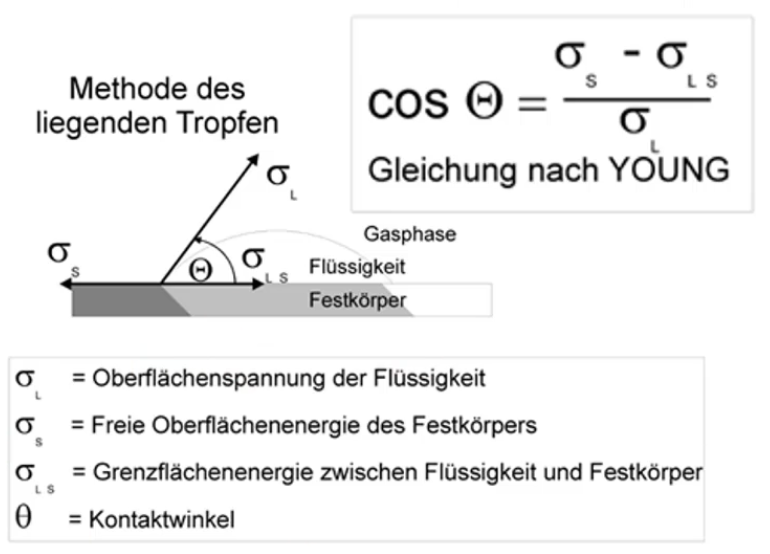
\includegraphics[width=8cm]{lec2/figures/young.png}	
\end{center}
\textbf{Neigungswinkel $\alpha$}\\
Neigungswinkel, ab welchem der Tropfen anfängt zu rollen. Weniger häufig angewandt zur Klassifizierung als Kontaktwinkel. 

\begin{center}
	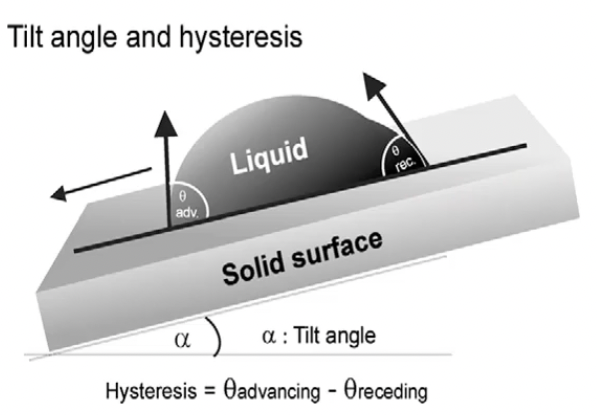
\includegraphics[width=8cm]{lec2/figures/neigungswinkel.png}	
\end{center}
Die Papillenartige Mikrostruktur beim Lotus-Blatt reduziert die effektive Fläche zwischen Flüssigkeit und Festkörper und beeinflusst dadurch die Grenzflächenenergie. Die folgenden \textbf{Typen des Benetzungsverhaltens} werden unterschieden \dangersign:

\begin{enumerate}
    \item \textbf{$\Theta < 90^\circ$}: hydrophil (benetzend)
    \item \textbf{$90^\circ < \Theta < 150^\circ$}: hydrophob (nicht benetzend)
    \item \textbf{$150^\circ \geq \Theta$}: superhydrophob
\end{enumerate}
Das Lotus-Blatt besitzt eine superhydrophobe Obefläche. Bei der Benetzung der verschiedenen Typen treten große dynamische Unterschiede bei der benetzenden Materie (z. B. Wasser) auf. 
\\\\
\textbf{Explizit klausurrelevant:} Einflussfaktoren des Benetzungsverhaltens \hintsign

\begin{itemize}
    \item Glatte vs. mikrostrukturierte Oberfläche
    \item Hydrophile vs. hydrophobe Oberfläche
    \item Oberflächenspannung des Wassers
    \item Kontaktfläche zwischen Tropfen und Oberfläche
    \item Lufteinschlüsse
\end{itemize}
\textit{Wie kommt es zustande, dass Strukturen superhydrophob sind und was muss erfüllt sein?}\\
Antwort: Mikrosturkutierung, Flüssigkeit muss passen, Oberfläche muss per se (chemisch) wasserabweisend sein.

\subsubsection{Der Selbstreinigungseffekt}

Der Selbstreinigungseffekt von Pflanzen ist \textbf{unabhängig von der Chemie} der Schmutzpartikel, setzt eine unbenetzbare Oberfläche voraus und wird durch folgende Zusammenhänge hervorgerufen \hintsign:

\begin{itemize}
    \item Reduzierte Kontaktfläche zwischen Pflanze und Partikeln durch \textbf{Mikrostrukturierung} (Haftkräfte von Partikeln auf Oberflächen auf 0,7 \% reduziert)
    \item \textbf{Unregelmäßige Strukturierung} reduziert die Kontaktfläche und die Haftkräfte weiter auf 0,07 \%
    \item Erhöhte Kontaktfläche der Partikel zum Wassertropfen
\end{itemize}

\begin{center}
	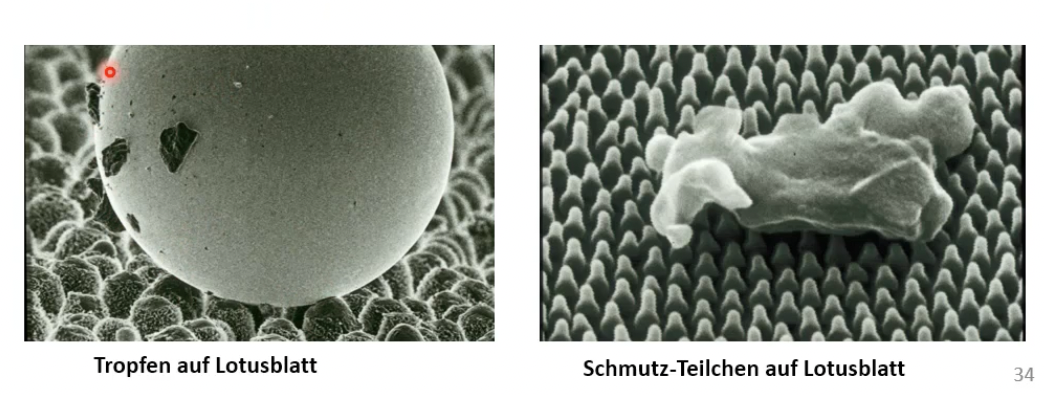
\includegraphics[width=12cm]{lec2/figures/selbstreinigung.png}	
\end{center}

\subsubsection{Herstellung von Papillen}

\textbf{Papillen} sind zapfenartige Vertiefungen und Erhebungen der Wachsschicht auf der Kutikula. Diese sind künstlich aufwändig herzustellen. In der Natur werden die Papillen vermutlich durch \textbf{Wachskristallbildung} konstruiert. Diese sind das Resultat von Selbstorganisationsprozessen und Wasserdampfdestillation über der Kutikula.

\begin{center}
	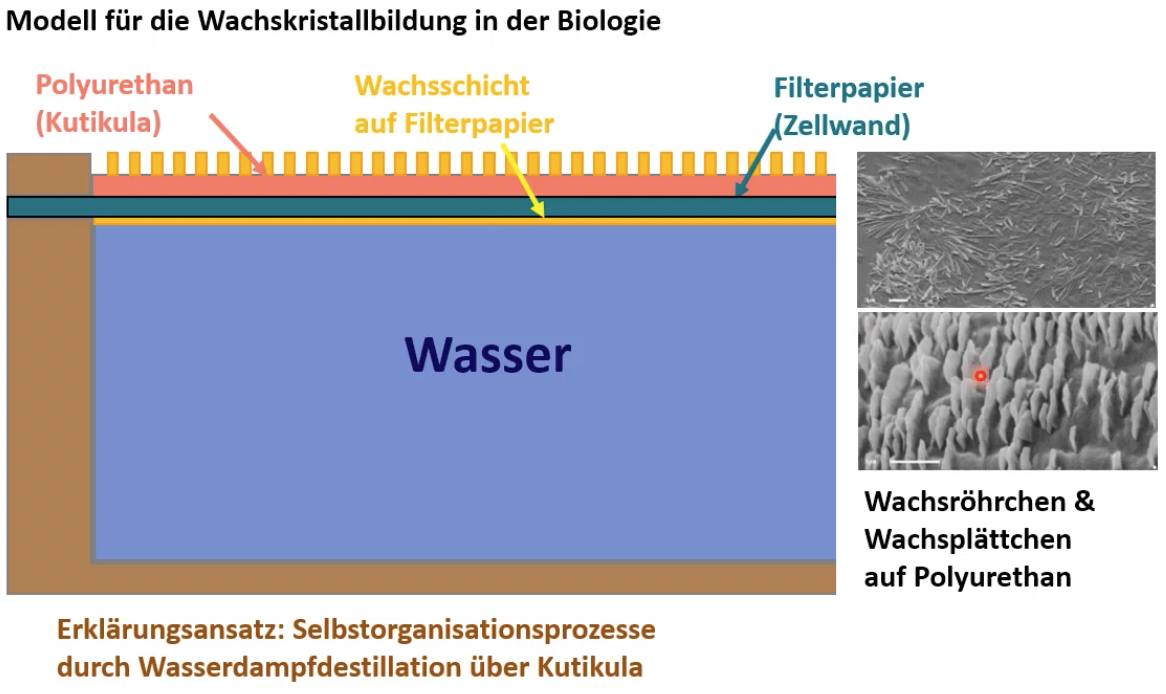
\includegraphics[width=12cm]{lec2/figures/wachskristallbildung.png}	
\end{center}
\subsubsection{Technische Anwendungen der Selbstreinigung - Der Lotus-Effekt}

Strukturen mit Lotus-Effekt sind immer \textbf{milchig} aufgrund der Papillen, welche das Licht unregelmäßig brechen und reflektieren. Herausforderungen entstehen durch Korrosion der künstlichen Wachsstrukturen, wodurch eine im Vergleich zu konventionellen Materialien vorzeitige Erneuerung notwendig wird, um den Effekt aufrechtzuerhalten. Dadurch meist kostenintensiver \dangersign. Bei der Pflanze wächst die Kutikula einfach nach, weshalb dies dort kein Problem darstellt.
\\\\
Anwendungsbeispiele für \textcolor{red}{selbstreinigende bzw. kontaktflächen-reduzierende künstliche Materialien} sind:

\begin{itemize}
    \item Fassadenfarbe mit Lotus-Effekt \dangersign
    \item Gläser (z.B.\ bei LKW-Mautsystem und Metallen)
    \item Sprays und Kunststoffbeschichtung (z.B.\ für Aufbewahrungsbehälter von teuren Flüßigkeiten)
    \item Textilien und Holzlacke (in Entwicklung)
    \item Honiglöffel (in Entwicklung)
    \item Dachziegel mit Titanoxid, das unter Einfluss von UV-Strahlung Elektronen freisetzt und Schmutz oxydiert (und dadurch zerstört)
    \item Kontaktflächenreduktion bei Hochtemperaturanwendungen (z.B.\ Bauteile in Hochöfen)
\end{itemize}

\subsection{Luftpolster unter Wasser}

Superhydrophobe Oberflächen bilden Luftkissen innerhalb der Papillen unter Wasser.
\\\\
Exkurs: Ein Beispiel für das Auftreten des Lotus-Effektes im Tierreich sind die \textbf{Sektrete und Drüsen von Streifenwanzen}, welche zur Feindabwehr und Abgabe von Pheromonen dienen sowie vor Mikroorganismen schützen. Da die Wanzen Luft über Tracheen (Vertiefungen über den ganzen Körper) aufnehmen und das Sekret auch für sie gitftig ist, müssen sie verhindern, dass es in die Tracheen gelangt. Die Lösung dafür ist ein gerichtetes und geführtes Abfließen über die Oberfläche, welches durch einen Lotus-Effekt erzielt wird.
\\\\
Die \textbf{unter Wasser glänzenden Luftpolster}, welche auf superhydrophobe Oberflächen schließen lassen, treten auch bei anderen Tierarten auf, wie z. B. der Südamerikanischen Wasserjagdspinne. Diese haben folgende Funktionen:

\begin{itemize}
    \item Schutzhülle gegen Feuchtigkeit und Temperatursprünge (vgl. Neoprenanzug)
    \item Versorgung mit Sauerstoff durch Tracheen-Atmung
\end{itemize}
In der Natur unterscheidet man die folgenden \textbf{drei Schwimmtypen}, welche teilweise aufgrund von Luftpolstern das Laufen auf dem Wasser erlauben:

\begin{enumerate}
    \item Passiv schwimmend (z. B. Schwimmfarn/ Salvinia)
    \item Aktive schwimmend (z. B. Wasserläufer)
    \item Tauchend (z. B. Wasserspinne)
\end{enumerate}
\textbf{Technische Anwendungen:}

\begin{itemize}
    \item Textilien für den Wassersport, die nicht nass werden \dangersign
    \item Beschichtung von Bootsrümpfen mit reibungsvermindernder Wirkung (reduzierter Strömungswiederstand)
\end{itemize}
\textbf{Fünf Prinzipien für permanente Luftschichten unter Wasser} \dangersign

\begin{enumerate}
    \item Hydrophobe Chemie
    \item Grobe Strukturen (z. B. Haare)
    \item Feinstruktur
    \item Hinterschneidung (damit Luftblasen  nicht aufgrund ihres Auftriebs entkommen)
    \item Elastizität (damit Luftblasen hinter Strukturen gehalten und nicht freigespült werden)
\end{enumerate}
Von diesen Prinzipien lassen sich die Feinstrukturen und Hinterschneidungen (Nanokavitäten) technisch nur äußerst schwer umsetzen. Es gelingt beispielsweise wasserabweisende Bademode herzustellen (hier können lediglich keine Feinstrukturen erzeugt werden).

\begin{center}
	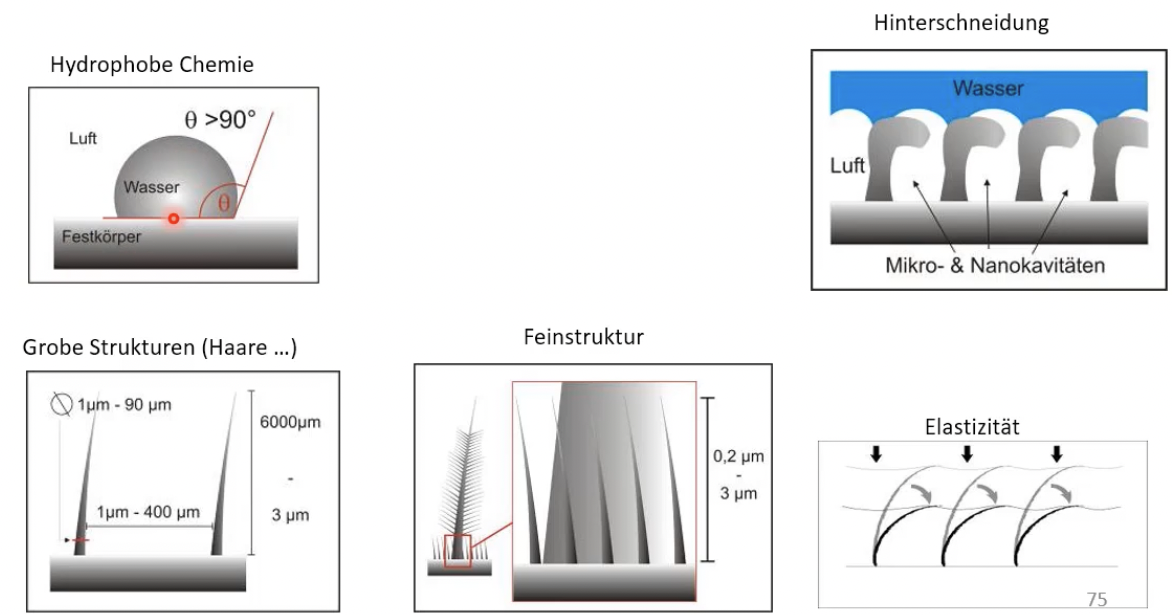
\includegraphics[width=14cm]{lec2/figures/prinizpien-luftschichten.png}	
\end{center}
Ein Prolbem, welches bei Luftpolstern unter Wasser auftreten kann, ist das sogennante \textbf{Salvinia-Problem}. Benannt ist es nach den verschiedenen Arten des Schwimmfarns von der Gattung Salvinia. Diese Pflanzen nutzen die Luftpolster, um ihre Blätter aufzuspannen und nahe der Wasseroberfläche zu halten (wo sie mehr Licht bekommen). Das Salvinia-Problem besteht darin, dass die Luft bei lokalen Druckinstabilitäten in Form von Luftblasen entweicht.
\\\\
Die Schwimmfarne der Gattung Salvinia verfügen außerdem über eine komplexe Zusammensetzung aus hydrophoben und hydrophilen Strukturen (an den Haarspitzen), wodurch sie sich an der Wasseroberfläche befestigen können. Dieser Effekt wird \textbf{Pinning} genannt.

\begin{center}
	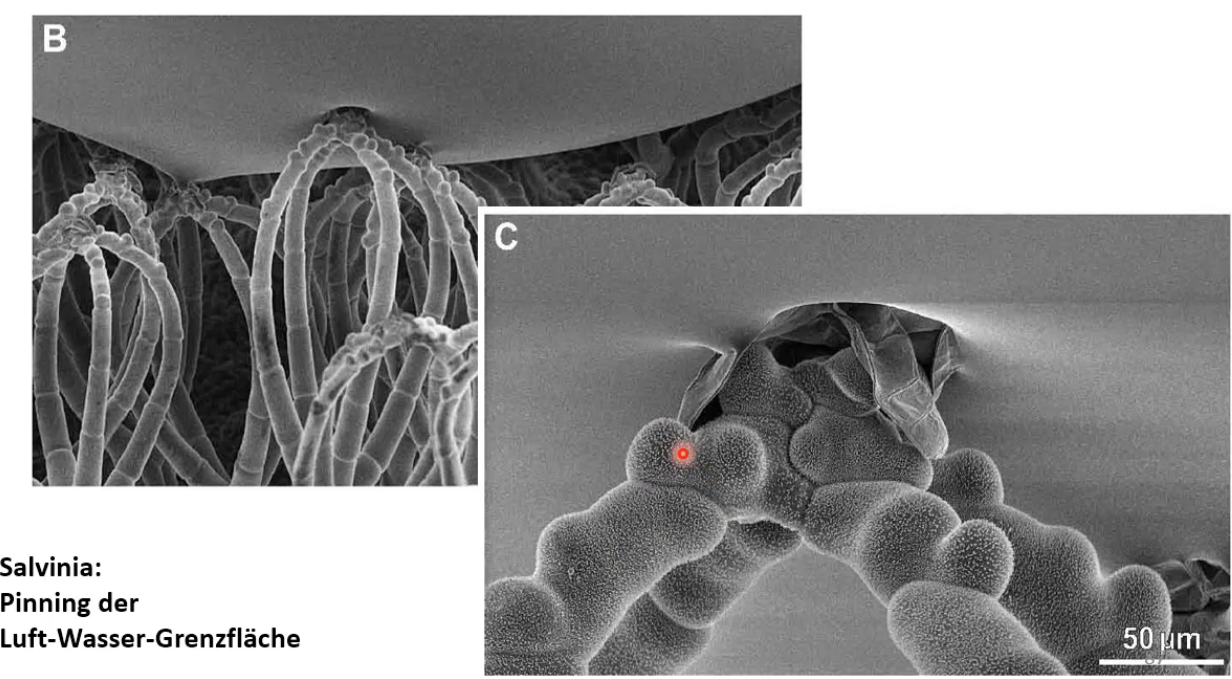
\includegraphics[width=14cm]{lec2/figures/pinning.png}	
\end{center}
Eine technische Anwendung stellt eine superhydrophobe Oberfläche für den Schiffsrumpf dar, die dann ein Luftpolster ausbildet (Salvinia-Effekt). Aktuell existieren auch z.B.\ Technologien, die dauerhaft Mikroluftblasen ausblasen, um Reibung zu verringern.

\subsection{Bionisches Antifouling: Bewuchsverhinderung im Meer}

Biogener (organischer) Bewuchs von Unterwasserkörpern durch Seepocken, Miesmuscheln und Algen verstärkt Korrosion und erhöht den Wasserwiederstand um bis zu 15 \%.
\\\\
Eine Lösung dafür aus der Natur ist ein \textbf{strukturiertes und elastisches System} nach Vorbild der Haihaut, welche aus Placoid-Schuppen besteht. Aus Experimenten mit unterschiedlich strukturierten und elastischen Gummi-Matten, welche im Meer versenkt wurden, wurde eine Haifischhaut-Farbe entwickelt, die \textbf{Bewuchs verringert} \dangersign.
\\\\
(\dangersign \textit{Welches Problem in der Schifffahrt? Was ist Antifouling? Was ist die konventionelle Lösung? Nenne eine Lösung aus der Bionik + Funktionsprinzip})










